\documentclass{ctexart}
\usepackage[utf8]{inputenc}
\usepackage{graphicx}
\usepackage{amsmath}
\usepackage{amssymb}
\usepackage{amsthm}
\usepackage{enumitem}
\usepackage{xcolor}
\usepackage{listings}
\newfontfamily\courier{Courier New}
\lstset{
    linewidth=1.1\textwidth,
    numbers=left, %设置行号位置 
    basicstyle=\small\courier,
    numberstyle=\tiny\courier, %设置行号大小  
    keywordstyle=\color{blue}\courier, %设置关键字颜色  
    %identifierstyle=\bf,
    commentstyle=\it\color[cmyk]{1,0,1,0}\courier, %设置注释颜色 
    stringstyle=\it\color[RGB]{128,0,0}\courier,
    %framexleftmargin=10mm,
    frame=single, %设置边框格式  
    backgroundcolor=\color[RGB]{245,245,244},
    %escapeinside=``, %逃逸字符(1左面的键),用于显示中文  
    breaklines, %自动折行  
    extendedchars=false, %解决代码跨页时,章节标题,页眉等汉字不显示的问题  
    xleftmargin=2em,xrightmargin=2em, aboveskip=1em, %设置边距  
    tabsize=4, %设置tab空格数  
    showspaces=false, %不显示空格  
    basicstyle=\small\courier,
}

\title{微分方程数值解 - 第九章理论作业}
\author{强基数学2001班樊睿}
\date{2023年3月29日}

\newtheorem{ex}{习题}
\newenvironment{sol}{\begin{proof}[\bf 解]}{\end{proof}}
\renewcommand{\proofname}{\bf 证明}

\begin{document}

\maketitle

\begin{ex}[9.5]
    证明近似解的相对误差由相对残量控制,即
    \begin{equation}
        \dfrac 1{\mathrm{cond}(A)} \dfrac {\Vert r\Vert_2}{\Vert b\Vert_2} \leq \dfrac {\Vert e\Vert_2}{\Vert x\Vert_2}\leq \mathrm{cond}(A) \dfrac {\Vert r\Vert_2}{\Vert b\Vert_2}.
    \end{equation}
\end{ex}

\begin{proof}
    因为 $Ae=r,A^{-1}r=e,Ax=b,A^{-1}b=x$,所以

    \begin{equation}
    \begin{split}
        & \dfrac 1{\mathrm{cond}(A)} \dfrac {\Vert r\Vert_2}{\Vert b\Vert_2} \\
        = & \dfrac 1{\Vert A\Vert_2\Vert A^{-1}\Vert_2}\dfrac {\Vert Ae\Vert_2}{\Vert b\Vert_2} \\
        \leq & \dfrac 1{\Vert A\Vert_2\Vert A^{-1}\Vert_2}\dfrac {\Vert A\Vert_2\Vert e\Vert_2}{\Vert b\Vert_2} \\
        = & \dfrac {\Vert e\Vert_2}{\Vert A^{-1}\Vert_2\Vert b \Vert_2}\\
        \leq & \dfrac {\Vert e\Vert_2}{\Vert x\Vert_2}.
    \end{split}
    \end{equation}

    另一方面,

    \begin{equation*}
    \begin{split}
        & \mathrm{cond}(A) \dfrac {\Vert r\Vert_2}{\Vert b\Vert_2} \\
        = & \Vert A\Vert_2\Vert A^{-1}\Vert_2\dfrac {\Vert r\Vert_2}{\Vert b\Vert_2} \\
        \geq & \Vert A\Vert_2\Vert A^{-1}\Vert_2\dfrac {\Vert r\Vert_2}{\Vert A\Vert_2\Vert x\Vert_2} \\
        = & \dfrac{\Vert A^{-1}\Vert_2\Vert r\Vert_2}{\Vert x\Vert_2} \\
        \geq & \dfrac {\Vert e\Vert_2}{\Vert x\Vert_2}.
    \end{split}
    \end{equation*}
\end{proof}

\begin{ex}[9.8]
    求一维 Dirichlet 边值问题的离散矩阵 $A$ 的条件数 $\mathrm{cond}(A)$ 在 $n=8$ 和 $n=1024$ 时的值。
\end{ex}

\begin{sol}
    根据 Lem 7.25 可得
    \begin{equation}
        \lambda_k(A) = \dfrac 4{h^2}\sin^2\dfrac{k\pi}{2(n+1)}.
    \end{equation}
    
    由条件数的定义,有
    
    \begin{equation}
        \mathrm{cond}(A) = \dfrac {\lambda_n(A)}{\lambda_1(A)} = \dfrac {\sin^2 \frac {(n-1)\pi}{2n}}{\sin^2 \frac {\pi}{2n}} = \tan^2 \dfrac{(n-1)\pi}{2n}
    \end{equation}
    
    当 $n=8$ 时,$\mathrm{cond}(A) = 25.27$.
    
    当 $n=1024$ 时,$\mathrm{cond}(A) = 424971.18$.
\end{sol}

\begin{ex}[9.11]
    对 $\Omega = (0,1)$,作图说明网格 $\Omega^h$ 上能表示的最多的波数为 $n_{\max} = \dfrac 1h$。如果 Fourier mode 在所有边界点处均为 $0$,情况如何?
\end{ex}

\begin{sol}
    以 $n=6,h=\dfrac 16$ 为例。

    \begin{figure}[htbp]
        \begin{minipage}{6cm}
            \centering
            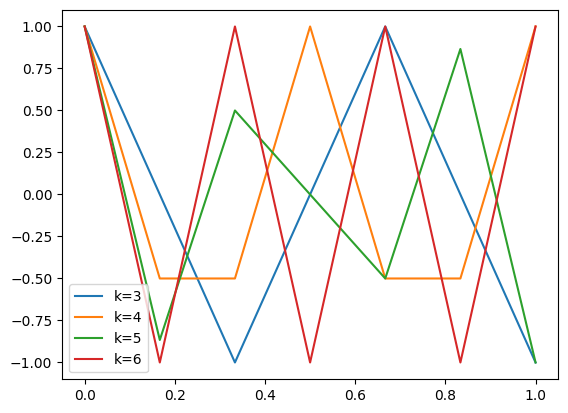
\includegraphics[width = 6cm, height = 4cm]{11-1.png}
            \caption{题9.11图-1}
            \label{9.11-fig1}
        \end{minipage}
        \qquad
        \begin{minipage}{6cm}
            \centering
            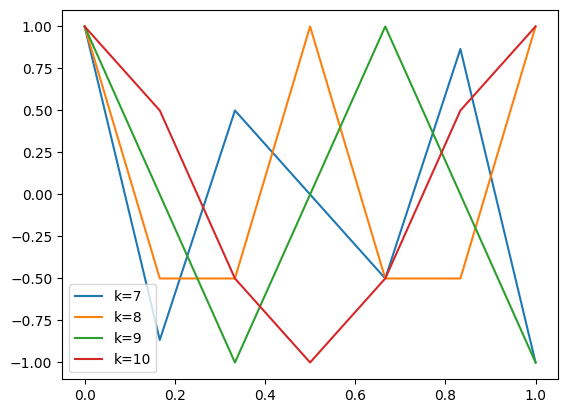
\includegraphics[width = 6cm, height = 4cm]{11-2.png}
            \caption{题9.11图-2}
            \label{9.11-fig2}
        \end{minipage}
    \end{figure}

    通过作出 $y=\cos(k\pi x)$ 在 $k=3,4,\dots,10$ 的图像(如\ref{9.11-fig1}、\ref{9.11-fig2}所示),可知:$k\leq n$ 时,网格上显示的波数和实际波数相同;$k>n$ 时,网格上显示的波数为 $2n-k$。

    若要求边界点处的值为 $0$,则当 $k=n$ 时网格点处的值也均为 $0$。这时是不能显示出 $n$ 个半波的。此时最多只能显示出 $n-1$ 个半波。
\end{sol}

\begin{ex}[9.14]
    作出 Example 9.13 的 $n=6$ 情形的图。
\end{ex}

\begin{sol}

作图代码如下:

\begin{lstlisting}[language={python}]
N = 1000
n = 6
k1 = n*0.5
k2 = n*1.5

def w(k, x) :
    return math.sin(k*pi*x)

xx = [i/N for i in range(N+1)]
yy1 = [w(k1,t) for t in xx]
yy2 = [w(k2,t) for t in xx]

x = [i/n for i in range(n+1)]
y1 = [w(k1,t) for t in x]
y2 = [w(k2,t) for t in x]

plt.plot(xx,yy1)
plt.plot(xx,yy2)
plt.plot(x,y1)
plt.plot(x,y2)
\end{lstlisting}

画出 $y=\sin \dfrac n2 x$ 和 $y=\sin \dfrac {3n}2 x$ 的图像,以及仅利用格点处的值线性插值的图像,如图\ref{9.14-fig}所示。

\begin{figure}[h]
	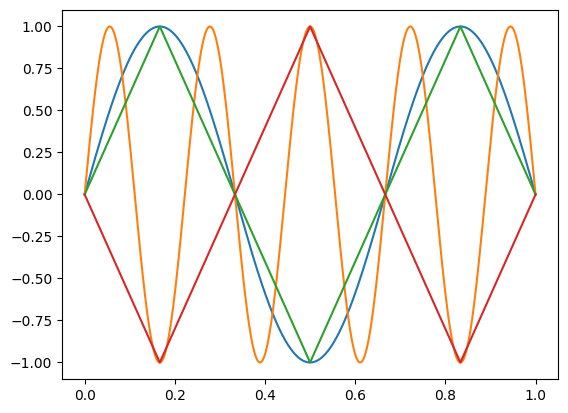
\includegraphics[width = 12cm, height = 8cm]{14.png}
    \caption{题 9.14 图}
	\label{9.14-fig}
\end{figure}

由图\ref{9.14-fig}可知,虽然两条曲线本身波数不同,但在 $n=6$ 的网格上都只能描述出 $\dfrac n2=3$ 个半波。
\end{sol}

\begin{ex}[9.17]

对一维 Dirichlet 边值问题的线性系统 $Au=f$ 证明加权 Jacobi 迭代的迭代矩阵,证明

\begin{equation}
    T_\omega = (1-\omega)I + \omega D^{-1}(L+U) = I - \dfrac {\omega h^2}2 A,
\end{equation}

其特征向量和 $A$ 的相同,特征值为

\begin{equation}
    \lambda_k(T_\omega) = 1 - 2\omega \sin^2 \dfrac {k\pi}{2n}.
\end{equation}

\end{ex}

\begin{proof}
根据迭代矩阵的公式,有
\begin{equation}
\begin{split}
    T_w & = (1-\omega)I + \omega D^{-1}(L+U) \\
        & = (1-\omega)I + \omega D^{-1}(L+U-D) + \omega I \\
        & = I - \omega D^{-1}A \\
\end{split}
\end{equation}
其中第三个等号是因为 $A = D-L-U$。

因为 $A$ 的对角线元素全是 $\dfrac 2{h^2}$,所以 $D = \dfrac 2{h^2}I$,$D^{-1} = \dfrac {h^2}2I$。

因此

\begin{equation}
    T_{\omega} = I - \dfrac {\omega h^2}2 A.
\end{equation}

设 $v_k$ 是对应 $A$ 的特征值 $\lambda_k$ 特征向量。则

\begin{equation}
    T_\omega v_k = (1 - \dfrac{\omega h^2}2 A)v_k
                 = v_k - \dfrac{\omega h^2}2 Av_k
                 = v_k - \dfrac{\omega h^2}2 \lambda_kv_k
                 = (1 - \dfrac{\omega h^2}2\lambda_k)v_k
\end{equation}

因此 $v_k$ 是对应 $T_\omega$ 的特征值 
\begin{equation}
    1 - \dfrac{\omega h^2}2\lambda_k
    = 1 - \dfrac{\omega h^2}2\dfrac 4{h^2}\sin^2\dfrac {k\pi}{2n}
    = 1 - 2\omega \sin^2\dfrac{k\pi}{2n}
\end{equation}
的特征向量。
\end{proof}

\begin{ex}[9.18]
    用程序作出 Fig. 2.7 by Briggs et al. [2000]. $n=64,\omega\in [0,1]$。证明 $\rho(T_\omega)\geq 0.9986$,即收敛速度缓慢。
\end{ex}

\begin{sol}

作图代码如下:

\begin{lstlisting}
n = 64
def lmd(w, k) :
    return 1 - 2 * w * math.sin(k*pi / (2*n)) ** 2

plt.xlabel('k')
plt.ylabel('eigenvalue')
plt.plot([0,64],[0,0])
ks = [k for k in range(1,n)]
for w in [1/3, 1/2, 2/3, 1]:
    ls = [lmd(w, k) for k in ks]
    plt.plot(ks, ls, label = "w={:f}".format(w))
plt.legend()
\end{lstlisting}

结果如图 \ref{9.18-fig1} 所示。

\begin{figure}[h]
    \centering
	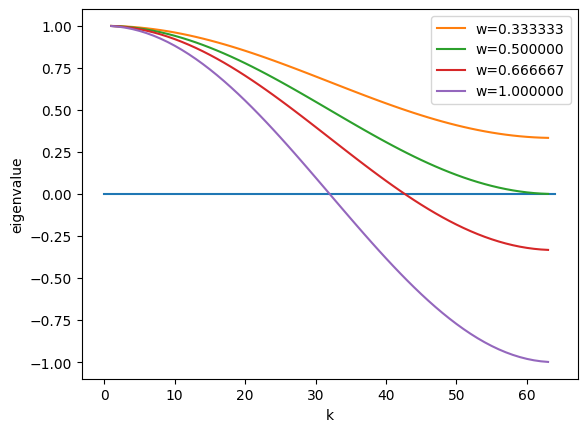
\includegraphics[width = 12cm, height = 8cm]{18.png}
    \caption{题9.18图}
	\label{9.18-fig1}
\end{figure}

当 $n=64,\omega\in (0,1)$ 时,

\begin{equation}
    \rho(T_{\omega}) = \lambda_{\max} > 1 - 2\sin^2 \dfrac{\pi}{2n} \approx 0.998795.
\end{equation}

根据迭代法收敛速度的性质,因为 $\rho(T_{\omega})\rightarrow 1$,所以收敛速度缓慢。

\end{sol}

\begin{ex}[9.21]
    用程序作出 Fig. 2.8 by Briggs et al. [2000]. 证明常规Jacobi方法只在 $16\leq k\leq 48$ 的模式是良好的。反之,对于 $\omega = \dfrac 13$,证明对 $16\leq k<64$ 均是良好的。
\end{ex}

\begin{sol}
作图代码如下:
\begin{lstlisting}
n = 64

def lmd(w, k) :
    return 1 - 2 * w * math.sin(k*pi / (2*n)) ** 2
def itnum(w, k) :
    return min(100, math.log(0.01) / math.log(abs(lmd(w, k))))

plt.xlabel('k')
plt.ylabel('iteration times')
ks = [k for k in range(1,n)]
for w in [1, 2/3]:
    ls = [itnum(w, k) for k in ks]
    plt.plot(ks, ls, label = "w={:f}".format(w))
plt.legend()
\end{lstlisting}

结果如图 \ref{9.21-fig1} 所示。

\begin{figure}[h]
    \centering
	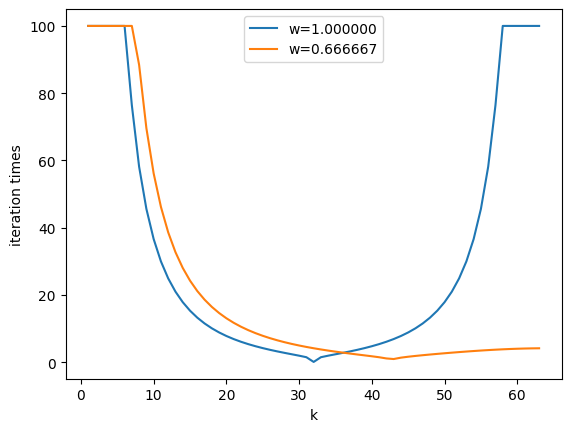
\includegraphics[width = 12cm, height = 8cm]{21.png}
    \caption{题9.21图}
	\label{9.21-fig1}
\end{figure}

蓝色和黄色曲线分别是 $\omega=1$(即不加权的Jacobi方法)和 $\omega=\dfrac 23$ 时迭代次数关于 $k$ 的函数图像。

同样使精度增加两位,不加权的Jacobi方法的迭代次数在 $16\leq k\leq 48$ 时都很小(不超过 $15$ 次),在 $k$ 较小或较大时迭代次数都会很大;加权的Jacobi方法在 $\omega=\dfrac 23$ 时,只要 $k\geq 16$,迭代次数都不超过 $15$ 次,且当 $k\geq 32$ 时迭代次数非常少,只需最多 $5$ 次。

这是因为,对于不加权的Jacobi方法,当 $16\leq k\leq 48$ 时,$\sin\dfrac{k\pi}{2n}\in[\sqrt{1-\dfrac{\sqrt 2}2},\sqrt{1+\dfrac{\sqrt 2}2}]$,$\lambda_k = 1-2\sin^2\dfrac{k\pi}{2n}\in [1-\sqrt 2, \sqrt 2-1]$,快速收敛;

对于加权Jacobi方法,当 $k\geq 32=\dfrac n2$ 时,$\sin\dfrac{k\pi}{2n}\in[\dfrac 1{\sqrt 2},1)$,$\lambda_k = 1-2\omega\sin^2\dfrac{k\pi}{2n} \in (-\dfrac 13,\dfrac 13]$,快速收敛。

\end{sol}

\begin{ex}[9.35]
    证明对于 $\nu_1=\nu_2=1$,FMG的计算代价小于 $\dfrac 2{(1-2^{-\mathrm{D}})^2}\mathrm{WU}$。给出FMG当 $\mathrm{D}=1,2,3$ 时尽可能紧的上界。
\end{ex}

\begin{sol}
    先考虑FMG-3(即VC循环)的执行次数。VC循环要在宽度为 $h,2h,2^2h,\dots,2^{m-1}h$ 的网格上各进行一次,每次花费的代价为
    \begin{equation}
        2(2^{-k\mathrm{D}}+2^{-(k+1)\mathrm{D}}+ \cdots +2^{-m\mathrm{D}})\mathrm{WU} < \dfrac{2^{-k\mathrm{D}+1}}{1-2^{-\mathrm{D}}}\mathrm{WU}.
    \end{equation}
    其中,$k=1,2,\dots,m$。

    这样,VC循环的总代价就是
    \begin{equation}
        \dfrac 2{1-2^{-\mathrm{D}}}(2^{-\mathrm{D}}+2^{-2\mathrm{D}}+\cdots+2^{-m\mathrm{D}})\mathrm{WU} < \dfrac {2^{-\mathrm{D}+1}}{(1-2^{-\mathrm{D}})^2}\mathrm{WU}.
    \end{equation}

    又因为FMG-1和FMG-2在每种宽度的网格上也都会执行一次,所以这部分的代价为
    \begin{equation}
        2(1+2^{-\mathrm{D}}+2^{-2\mathrm{D}}+\cdots+2^{-m\mathrm{D}})\mathrm{WU} = \dfrac 2{1-2^{-\mathrm{D}}}\mathrm{WU}.
    \end{equation}

    总代价为

    \begin{equation}
        \dfrac {2(2^{-\mathrm{D}}+1-2^{-\mathrm{D}})}{(1-2^{-\mathrm{D}})^2}\mathrm{WU} = \dfrac 2{(1-2^{-\mathrm{D}})^2}\mathrm{WU}.
    \end{equation}

    当 $\mathrm{D} = 1,2,3$ 时,分别有上界 $8\mathrm{WU},\dfrac {32}9\mathrm{WU},\dfrac {128}{49}\mathrm{WU}$。
\end{sol}

\begin{ex}
    将 (9.32) 重写为

    \begin{equation}
        TG
        \begin{bmatrix}
            w_k
            \\
            w_{k'}
        \end{bmatrix}
        = 
        \begin{bmatrix}
            \lambda_k^{\nu_1+\nu_2}s_k & \lambda_k^{\nu_1}\lambda_{k'}^{\nu_2}s_k\\
            \lambda_{k'}^{\nu_1}\lambda_k^{\nu_2}c_k & \lambda_{k'}^{\nu_1+\nu_2}c_k
        \end{bmatrix}
        \begin{bmatrix}
            w_k
            \\
            w_{k'}
        \end{bmatrix}
        =
        \begin{bmatrix}
            c_1 & c_2 \\
            c_3 & c_4 \\
        \end{bmatrix}
        \begin{bmatrix}
            w_k
            \\
            w_{k'}
        \end{bmatrix}
    \end{equation}
    解释 $c_i$ 很小的原因。通过作出双网格校正 $n=64,\omega = \dfrac 23$ 情形对应不同衰减系数的的六个图像,导出 $\rho(TG)\approx 0.1$ 的结论。对 $n=128$ 作同样的图,证明 $\rho(TG)$ 与 $n$ 的大小无关。
\end{ex}

\begin{sol}
作图代码如下:

\begin{lstlisting}
n = 64
w = 2/3

def lmd(w, k) :
    return 1 - 2 * w * math.sin(k*pi / (2*n)) ** 2

def c(k) :
    return math.cos(k*pi/(2*n))**2+

def s(k) :
    return math.sin(k*pi/(2*n))**2

k1s = [k for k in range(1,n//2+1)]
k2s = [k for k in range(n//2, n)]

id = 0
for [v1,v2] in [[0,0],[0,2],[1,1],[2,0],[2,2],[4,0]]:
    id += 1
    plt.figure(id)
    plt.xlabel('k')
    plt.ylabel('coefficients')
    c1s = [lmd(w, k) ** (v1+v2) * s(k) for k in range(1, n//2+1)]
    c2s = [lmd(w, n-k) ** v1 * lmd(w, k) ** v2 * s(n-k) for k in range(1, n//2+1)]
    c3s = [lmd(w, n-k) ** v1 * lmd(w, k) ** v2 * c(k) for k in range(n//2, n)]
    c4s = [lmd(w, k) ** (v1+v2) * c(n-k) for k in range(n//2, n)]
    plt.plot(k1s, c1s, label = 'c1')
    plt.plot(k1s, c2s, label = 'c2')
    plt.plot(k2s, c3s, label = 'c3')
    plt.plot(k2s, c4s, label = 'c4')
    plt.legend()
\end{lstlisting}

作图结果如图 \ref{9.41-fig1} 至 \ref{9.41-fig6} 所示。$\rho(TG)$ 是图中 $\rho$ 曲线的极大值。

\begin{figure}[htbp]
    \begin{minipage}{6cm}
        \centering
        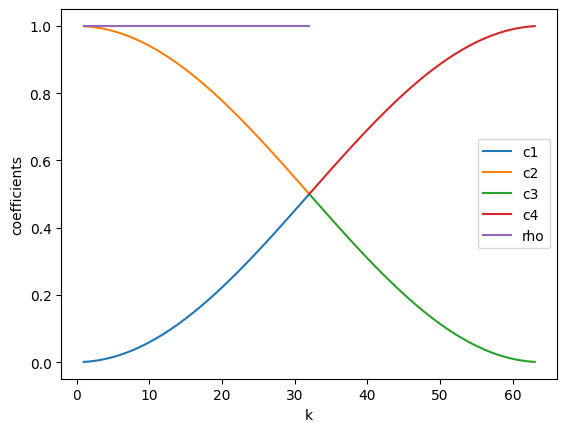
\includegraphics[width = 6cm, height = 4cm]{41-1.png}
        \caption{$\nu_1=0,\nu_2=0$}
        \label{9.41-fig1}
    \end{minipage}
    \qquad
    \begin{minipage}{6cm}
        \centering
        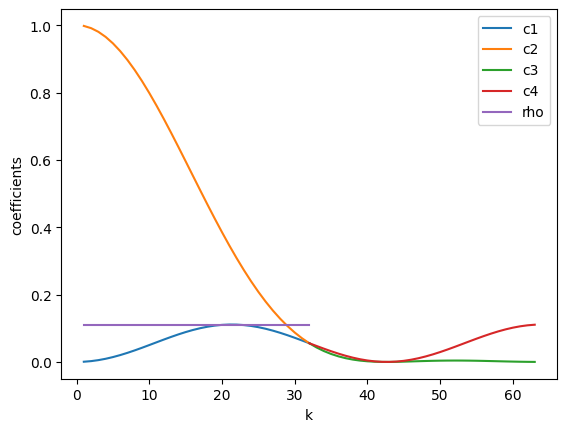
\includegraphics[width = 6cm, height = 4cm]{41-2.png}
        \caption{$\nu_1=0,\nu_2=2$}
        \label{9.41-fig2}
    \end{minipage}

    \begin{minipage}{6cm}
        \centering
        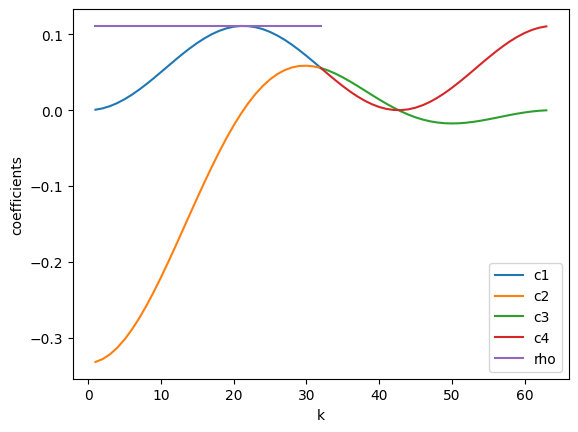
\includegraphics[width = 6cm, height = 4cm]{41-3.png}
        \caption{$\nu_1=1,\nu_2=1$}
        \label{9.41-fig3}
    \end{minipage}
    \qquad
    \begin{minipage}{6cm}
        \centering
        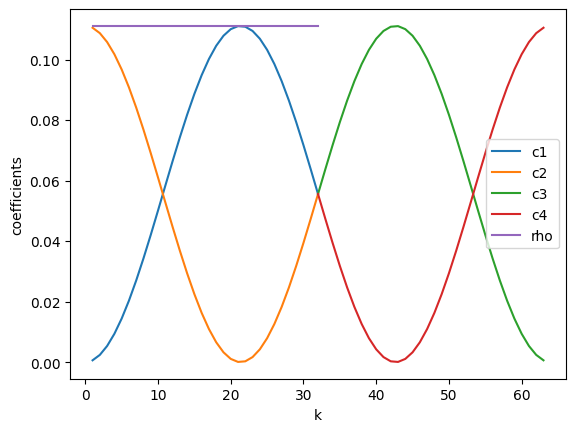
\includegraphics[width = 6cm, height = 4cm]{41-4.png}
        \caption{$\nu_1=2,\nu_2=0$}
        \label{9.41-fig4}
    \end{minipage}

    \begin{minipage}{6cm}
        \centering
        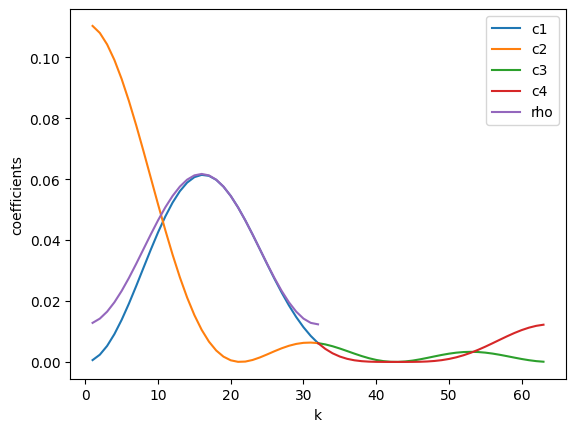
\includegraphics[width = 6cm, height = 4cm]{41-5.png}
        \caption{$\nu_1=2,\nu_2=2$}
        \label{9.41-fig5}
    \end{minipage}
    \qquad
    \begin{minipage}{6cm}
        \centering
        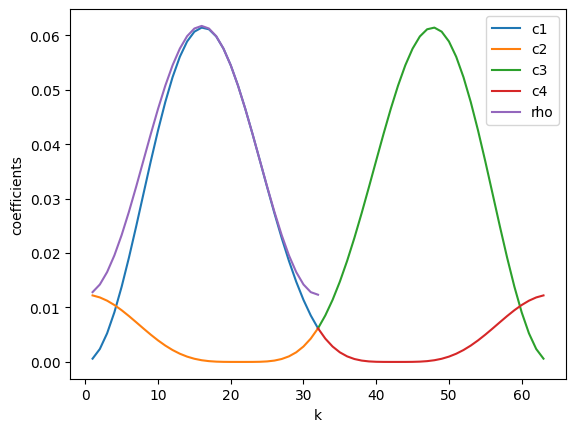
\includegraphics[width = 6cm, height = 4cm]{41-6.png}
        \caption{$\nu_1=4,\nu_2=0$}
        \label{9.41-fig6}
    \end{minipage}
\end{figure}

由此可见,当 $\nu_1\neq 0$ 或 $\nu_2\neq 0$ 时,均有 $\rho(TG)\leq 0.1$。进一步当 $\nu_1=2,\nu_2=2$ 或 $\nu_1=4,\nu_2=0$ 时,$\rho(TG) \approx 0.06$。

将 $n$ 改为 $128$,得到图 \ref{9.41-fig7} 到图 \ref{9.41-fig12}。

\begin{figure}[htbp]
    \begin{minipage}{6cm}
        \centering
        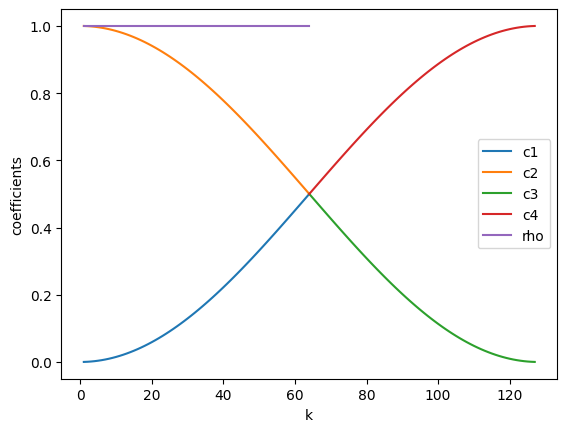
\includegraphics[width = 6cm, height = 4cm]{41-7.png}
        \caption{$\nu_1=0,\nu_2=0$}
        \label{9.41-fig7}
    \end{minipage}
    \qquad
    \begin{minipage}{6cm}
        \centering
        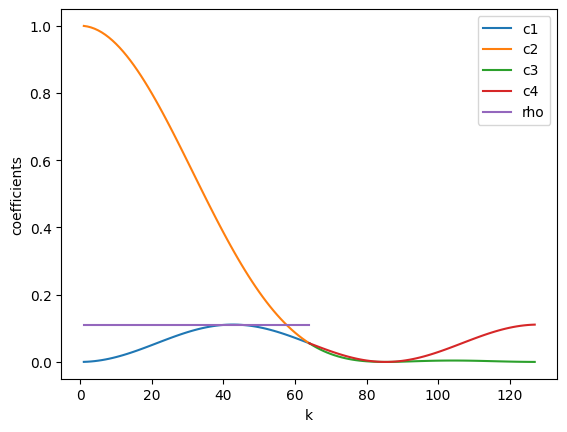
\includegraphics[width = 6cm, height = 4cm]{41-8.png}
        \caption{$\nu_1=0,\nu_2=2$}
        \label{9.41-fig8}
    \end{minipage}

    \begin{minipage}{6cm}
        \centering
        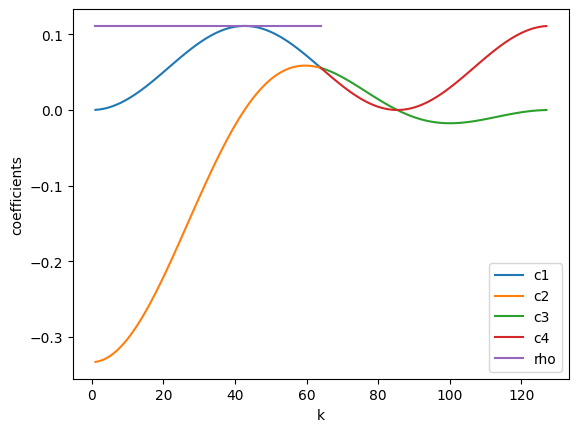
\includegraphics[width = 6cm, height = 4cm]{41-9.png}
        \caption{$\nu_1=1,\nu_2=1$}
        \label{9.41-fig9}
    \end{minipage}
    \qquad
    \begin{minipage}{6cm}
        \centering
        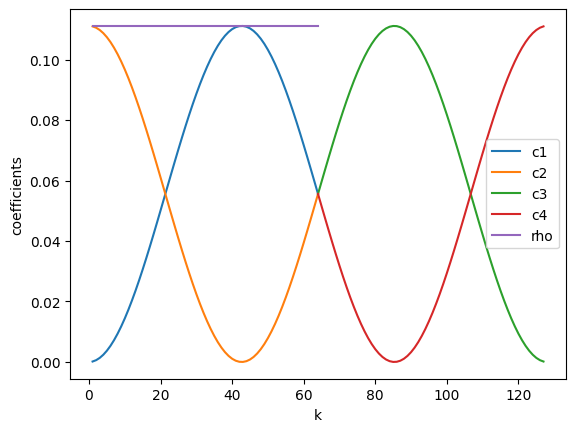
\includegraphics[width = 6cm, height = 4cm]{41-10.png}
        \caption{$\nu_1=2,\nu_2=0$}
        \label{9.41-fig10}
    \end{minipage}

    \begin{minipage}{6cm}
        \centering
        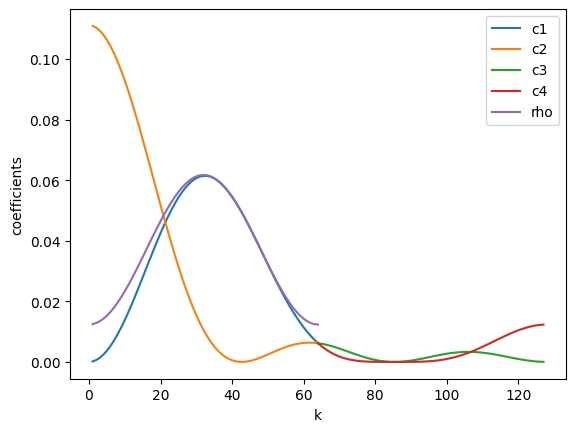
\includegraphics[width = 6cm, height = 4cm]{41-11.png}
        \caption{$\nu_1=2,\nu_2=2$}
        \label{9.41-fig11}
    \end{minipage}
    \qquad
    \begin{minipage}{6cm}
        \centering
        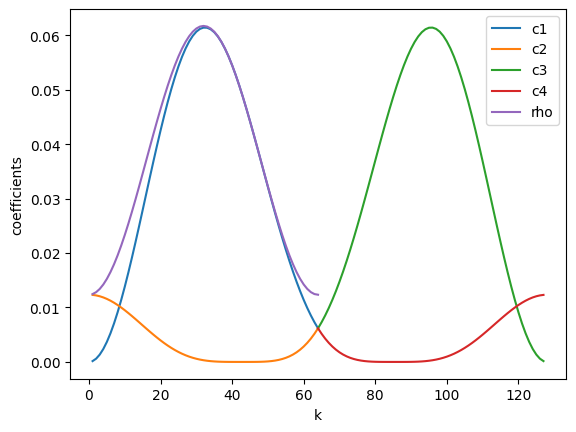
\includegraphics[width = 6cm, height = 4cm]{41-12.png}
        \caption{$\nu_1=4,\nu_2=0$}
        \label{9.41-fig12}
    \end{minipage}
\end{figure}

可见把 $n$ 改为 $128$ 后,$c_1,c_2,c_3,c_4,\rho$ 的值域都不变。事实上它们的图像相比 $n=64$ 只是水平方向拉长到原来的 $2$ 倍。显然 $\rho(TG)$ 也不变。

\end{sol}

\begin{ex}
    证明全加权算子满足
    \begin{equation}
        \dim \mathcal{R}(I_h^{2h}) = \dfrac n2-1,\dim \mathcal{N}(I_h^{2h}) = \dfrac n2.
    \end{equation}
\end{ex}

\begin{sol}
    因为 $I_h^{2h}$ 是行满秩的,所以
    \begin{equation}
        \dim \mathcal{R}(I_h^{2h}) = \mathrm{rank}(I_h^{2h}) = \dfrac n2-1.
    \end{equation}
    
    根据线性映射基本定理,
    \begin{equation}
        n-1 = \dim R^{n-1} = \dim \mathcal{R}(I_h^{2h}) + \dim \mathcal{N}(I_h^{2h}).
    \end{equation}

    所以
    \begin{equation}
        \dim \mathcal{N}(I_h^{2h}) = (n-1) - \mathcal{R}(I_h^{2h}) = (n-1) - (\dfrac n2-1) = \dfrac n2.
    \end{equation}
\end{sol}

\end{document}